\chapter{Entwurf und Implementierung}
\label{cha:implementierung}

\todo{Kapitel-Einleitung}



\section{Modularer Architektur-Vorschlag}

%Komponenten des Brokers.
%
%
%In der CMP: Polling oder Notification?
%
%Was löst eine Aktion aus?
%- Monitoring der Services
%- Änderung der Umgebung
%- User-Aktion
%- Ergebnis einer anderen Policy

\begin{figure}
	\centering	
%	\def\svgwidth{0.95\textwidth}
%	{\tiny
%	\includesvg{images/broker-cycle}}
	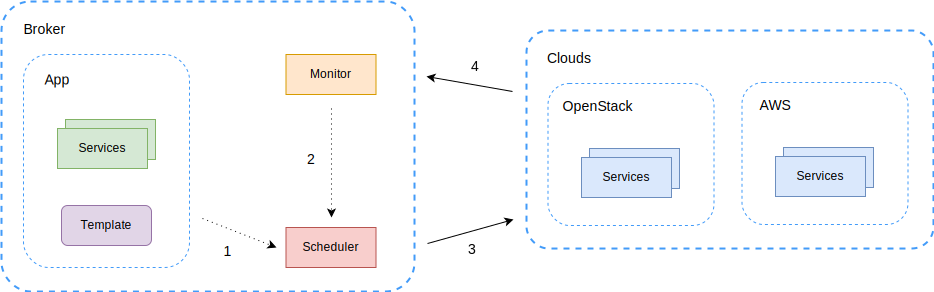
\includegraphics[width=\linewidth]{images/broker-cycle}
	\caption{Arbeitsweise des Multi-Cloud-Brokers als Zyklus: (1) Sammeln der Meta-Informationen aller Cloud-Provider, (2) Sammeln der Laufzeitinformationen der Anwendungen, (3) Sammeln der SLAs, (4) Nutzeränderungen: Neue Anwendungen oder Anpassung von SLAs, (5) Optimierungsplanung, (6) Planausführung auf den Cloud-Infrastrukturen}
	\label{fig:cycle}
\end{figure}

%Zyklus\autoref{fig:cycle}:

%\begin{description}
%	\item[Nummerierte Aufzählung]~\par
\begin{enumerate}
	
	\item Sammeln der Meta-Informationen alle Cloud-Provider
	\begin{enumerate}
		\item Kapazität (CPU, RAM, HDD, Network)
		\item Features (Verschlüsselung, CUDA, …)
		\item Geo-Lokation 
		\item Preis
	\end{enumerate}
	
	\item Sammeln der Laufzeitinformationen der PaaS/Anwendungen
	\begin{enumerate}
		\item Auslastung
		\item Fehler
		\item Ausfälle
	\end{enumerate}
	
	\item Sammeln der SLAs
	\begin{enumerate}
		\item Policy-Definitionen
		\item Policy-Konfiguration
		\item Placement-Algorithmen
	\end{enumerate}
	
	\item Neue Anwendung/Änderung eines SLA
	
	\item Optimierung
	\begin{enumerate}
		\item Feste Vorgaben (Geo, Backup)
		\item Weiche (Preis, Latenz, Verfügbarkeit)
	\end{enumerate}
	
	
	\item Ausführung
	\begin{enumerate}
		\item Netzwerkkonfiguration
		\item Allokation/De-Allokation von Ressourcen
		\item Deployment
		\item Migration
		\item Logging/Benachrichtigung
		\item Backup
	\end{enumerate}
	
\end{enumerate}

\section{Brokering}


%https://de.wikipedia.org/wiki/Constraintprogrammierung
%https://de.wikipedia.org/wiki/Scheduling

%entailing multiple constraint satisfaction (MCS)
%
%\todo{Schaubild, was wird wann gematcht}
%% Pseudocode des Algorithmus, wie in Meryn
%
%Kostenoptimierung
%
%Preisentwicklung? 
%
%Migration je nach Tageszeit? 
%
%Kosten der Datentransfers 
%
%Subscription On-Demand/Monthly/Yearly 
%
%Kompliziert durch undurchsichtige Staffelpreise
% https://www.rightscale.com/blog/cloud-cost-analysis/aws-vs-azure-vs-google-cloud-pricing-compute-instances

%https://www.rightscale.com/blog/cloud-cost-analysis/comparing-cloud-instance-pricing-aws-vs-azure-vs-google-vs-ibm

%
%Cost Calculators 
%
%http://go.appscale.com/cloud-cost-calculator-help 
%
%https://github.com/ifosch/accloudtant 
%
%https://awstcocalculator.com/# 
%

\section{Testanwendung: Hyrise-R}

Hyrise\footnote{\url{https://hpi.de/plattner/projects/hyrise.html}} ist eine In-Memory-Forschungsdatenbank der Fachgruppe \emph{Enterprise Platform and Integration Concepts (EPIC)} am Hasso-Plattner-Institut \cite{grund:2010:hyrise}. Die Datenbank teilt sich einige Eigenschaften mit \emph{SAP HANA}\footnote{\url{https://www.sap.com/products/hana.html}}: Ein \emph{Delta Store}, spaltenorientierte Speicherung, Wörterbuchkodierung und weitere Komprimierungstechniken sowie den \emph{Insert-Only}-Ansatz und Partitionierung. Herausragend ist die OLAP-Performance, enthalten sind aber auch Optimierungen für OLTP-Aufgaben.

Hyrise-R ist eine Erweiterung des Basisprojektes um Replikation \cite{schwalb:2015:hyrise-r}. Es folgt dabei dem \emph{Scale-Out}-Ansatz: Alle schreibenden Operationen werden auf einem einzigen \emph{Master-Node} durchgeführt. Dessen Datensatz wird in weniger als einer Sekunde (\emph{lazy}) mit beliebig vielen \emph{Replica-Nodes} abgeglichen. Diese Spiegelungen bearbeiten alle reinen Leseanfragen und machen den Verbund so skalierbar, siehe \autoref{fig:hyrise-r}. Nach dem \emph{CAP-Theorem} sind Verfügbarkeit und Partitionstoleranz hier also wichtiger als Konsistenz. 

\begin{figure}[ht]
	\centering
	\def\svgwidth{0.9\textwidth}
	\textsf{
	\includesvg{images/hyrise-r}}
	\caption{Verteilte \emph{Hyrise-R}-Architektur mit getrennter Verarbeitung von Lese- und Schreibanfragen. Der Master-Knoten dient als \emph{Single Source of Truth}. Zur Leistungssteigerung übernehmen Spiegelserver die Beantwortung der meisten Leseanfragen. Kleinere Inkonsistenzen werden dabei in Kauf genommen. Nicht im Bild ist der Dispatcher zur Anfrageverteilung. Aus \cite{ssiclops:d42:experiments-measurements}.}	
	\label{fig:hyrise-r}
\end{figure}

Durch die verteilte Architektur ist Hyrise-R ein potenzieller Kandidat als Testanwendung innerhalb der Multi-Cloud-Umgebung. Einige \emph{SSICLOPS}-Teilprojekte untersuchten bereits Zuverlässigkeit, Performance, Datensicherheit und Vertraulichkeit in einer privaten OpenStack-Föderation \cite{ssiclops:d23:security-extensions, ssiclops:d42:experiments-measurements, bastian:2017:openstack-policies}. \todo{Diagramm:Hyrise-R on OS}

Im Rahmen dieser Arbeiten sind einige Infrastrukturteile als Code veröffentlicht: So existiert zum Beispiel eine Docker-Teststellung mit grafischem Cluster-Manager, um die Performance bei verschiedenen Replikationsstufen zu prüfen. Diese Infrastruktur wurde in mehreren Studienarbeiten weiter angepasst, um Hyrise-R-KVM-Images in OpenStack bereitzustellen \cite{eschrig:2016:ssiclops-masterproject, maschler:2017:ssiclops-masterproject}.

Um als Testanwendung über mehrere Cloud-Ebenen zu dienen, sollte Hyrise-R auf den verbreiteten Hypervisoren, IaaS- und CaaS-Providern ausführbar sein. Aufgrund der Softwarestruktur -- als eigenentwickelte \emph{Low-Level-C++-Anwendung} --  eignet Hyrise-R sich nicht direkt\footnote{\url{https://cloud.google.com/appengine/docs/flexible/custom-runtimes/}} als Testanwendung für die PaaS-Integration. Hierfür nutzen wir andere Standardsoftware, die auf den üblichen PaaS-Sprachen wie Java, Python oder Node.js aufbauen.

Hyrise-R ist von Anfang an für die Skalierung über externe Broker konzeptioniert. Die bisherigen Arbeiten haben \emph{Standalone-Cluster-Manager} umgesetzt, erst für Docker und später für OpenStack\footnote{\url{https://github.com/DukeHarris/hyrise_rcm}}\footnote{\url{https://github.com/SSICLOPS/openstack-testbed-vm}}. Die nötigen Clusterinformationen werden Hyrise-Instanzen direkt beim Start als Parameter übergeben. Variablen zur Laufzeitumgebung müssen während des Deployments vom Broker ausgefüllt werden: Konkret benötigt Hyrise einen TCP-Port und eine eindeutige Knoten-ID. Über ihre ID registrieren sich Knoten am Dispatcher. Hierzu benötigen sie dessen IP-Adresse und Port -- der Dispatcher muss also immer als Erstes in einem Cluster bereitstehen. Erst dann können Start und Registrierung des Masters erfolgen. Plattformunabhängig ergeben sich folgende Startskripte für einen Hyrise-R-Cluster:

\begin{description}
	
\item[{[1]} Dispatcher] einmal pro Cluster, zentrale Lastverteilung für alle Anfragen
	
\begin{minted}{jinja}
./dispatcher {{dispatcher.port}} settings.json
\end{minted}
	
\item[{[1]} Master] einmal pro Cluster als \emph{Single-Source-of-Truth}, bearbeitet alle Schreibanfragen, gekennzeichnet durch \emph{nodeId=0}
	
\begin{minted}{jinja}
./hyrise \
  --dispatcherurl={{dispatcher.ip}} \
  --dispatcherport={{dispatcher.port}} \
  --nodeId=0 \
  --port={{master.port}}
\end{minted}

\item[{[0-n]} Replica] optional, beliebig viele Instanzen pro Cluster zur Entlastung des Master-Knotens bei Leseanfragen

\begin{minted}{jinja}
./hyrise \
  --dispatcherurl={{dispatcher.ip}} \
  --dispatcherport={{dispatcher.port}} \
  --nodeId={{replica.id}} \
  --port={{replica.port}}
\end{minted}
	
\end{description}

\noindent
In vorherigen Projekten entwickelte Images für virtuelle Maschinen laufen auf der verbreiteten Hypervisorkombination aus QEMU und KVM. Die Erstkonfiguration erfolgte bisher über direkte SSH-Kommandos an die gestartete virtuelle Maschine. Dies erfordert die Konfiguration von SSH in den VMs und die Verwaltung von Schlüsseln in der CMP. Zusätzlich entsteht eine Wartezeit zwischen VM-Startkommando und Erstkonfiguration, die vorherige Projekte durch Polling noch ausdehnten. Eine elegantere Lösung ist \emph{cloud-init}: Die CMP füllt ein Konfigurationstemplate und schickt es direkt im Startkommando an den Infrastruktur-Provider. Dieser führt das Skript sofort ohne weitere Wartezeit aus.

Auch Docker-Images existieren bereits\footnote{\url{https://github.com/hyrise/hyrise-v1/tree/feature/docker}}, wurden aber seit 2015 nicht aktualisiert: Docker, diverse Abhängigkeiten und Hyrise selbst wurden in der Zwischenzeit weiterentwickelt. Innerhalb eines Clusters sollten alle Knoten dieselbe Hyrise-Version ausführen. Daher aktualisieren wir Dispatcher und Hyrise auf Basis des aktuellsten Hyrise-NVM-Branches\footnote{\url{https://github.com/janmattfeld/dispatcher/tree/docker}}\footnote{\url{https://github.com/janmattfeld/hyrise_nvm/tree/feature/docker}}.

Die Aktualisierung enthält das aktuelle Docker-Basis-Image Ubuntu 16.04. Wir integrieren außerdem korrekte Metadaten und Dokumentation zur Imageerstellung und Ausführung. Einige eingebundene Git-Submodule wurden in der Zwischenzeit verschoben oder existieren nicht mehr -- die verwendete CSV-Bibliothek muss zum Beispiel ausgetauscht werden. Dies erfordert kleinere Änderungen am Quellcode. Genauso wie neue \emph{Non-Uniform-Memory-Access-Funktionen (NUMA)}: Die Funktion \emph{membind} erfordert erweitere Rechte. In einem Standard-Docker-Container sind diese aber nicht vorhanden. Der neue Startparameter \mbox{\emph{-\,-disable\_membind}} deaktiviert die speziellen NUMA-Funktionen. Unsere Images laufen daher auch in Container-Laufzeitumgebungen der Public-Cloud-Provider.

Das Image ist zum Produktivbetrieb gedacht: Docker Build entfernt nach dem Image-Erstellungsprozess alle Abhängigkeiten, die zum Betrieb nicht notwendig sind. So reduziert sich die Image-Größe von über 500 auf weniger als 300\,MB -- entsprechend verkürzt sich die Startzeit. Enthalten ist außerdem eine Beispieldatenbank, die wir später als Benchmark und initialen Funktionstest nutzen werden. Gemessen wird also nicht die Synchronisationszeit der Hyrise-R-Lösung, sondern die Skalierungsfähigkeiten der verwendeten Cloud-Lösungen und Orchestrierungstechniken. Wir setzen außerdem pragmatische Startparameter für Hyrise-R auf Docker: \emph{-\,-corecount=2} \emph{-\,-disable\_membind}. Die neuen Images sind zur leichteren Integration auf Docker Hub veröffentlicht\footnote{\url{https://hub.docker.com/r/hyrise/dispatcher/}}\footnote{\url{https://hub.docker.com/r/janmattfeld/hyrise_r/}}. Um auch zukünftige Weiterentwicklungen von Hyrise nutzen zu können, automatisiert ein neues Makefile Docker-Build-Voränge und den Realease auf Docker Hub.

Aus der bisher losen Sammlung von Quellcode, Shell-Skripten und Makefiles in mehreren GitHub-Repositorys haben wir eine nachhaltige Pipeline zur automatisierten Image-Erstellung für verschiedene Infrastrukturen entwickelt\footnote{\url{https://github.com/janmattfeld/hyrise_nvm/commit/cfe3aa8}}. Ausführungsumgebung, Programm, Testdaten und Konfiguration werden flexibel integriert -- Hyrise-R eignet sich nun als Testanwendung für den Multi-Cloud-Broker.

Als Weiterentwicklung zu den bisherigen Hyrise-R-Arbeiten soll der Broker nicht nur nach Leistungsanforderungen skalieren, sondern auch SLAs und Geostandorte beachten sowie diverse Infrastrukturanbieter nutzen.


\input{content/4-4_openstack-testbed.tex}

\input{content/4-5_devstack-docker.tex}

\input{content/4-6_multi-cloud-bibliotheken.tex}


\section{Entwicklungsumgebung}

% Tatsächliche Broker Architektur
% Code-Eigenheiten
% Tests/KPIs/Validierung der Hypothese

\section{Softwarearchitektur}

%as in Grozev 42: Federated CLoud Management: There is a central repository of images. this is replicated to the specific iaas/caas providers on demand.
%
%Alle weiteren Managementprozesse sind für Clients transparent.


\section{Multi-Provider-Service-Schema}

% D2.1: Übersicht Policy-Sprachen: Performance und Speichergröße. Entgegengesetzte Interessen. Lesbarkeit über zweiteiliung: Einmal für Menschen, einmal auf Bit-ebene für Maschinen. SLA über Proxy

%D2.2: Policys auf allen Schichten

%Matthias Bastian: Policy in OpenStack.

...und SLAs.

Ziel: Portabilität.

Mensch-und maschinenlesbar

YAML als aktuellen Standard

%TOSCA komplex, aber vielversprechend. Hierauf aufbauen (eigenen YAML-Entwurf erwähnen) und Brokering hinzufügen. Hier muss festgelegt erden, welcher Service-Teil auf welchem Provider mit welchem Instanz-Typen bereitgestellt werden soll. Dies soll automatisiert anhand von SLA/Policy und Preis entschieden werden. Unterstützt TOSCA deklarative Service-Definitionen?
%
%
%TOSCA hat folgendes nur optional
%- YAML (als SimpleVersion)
%- Multi-Provider als Plugin (nicht gewartet)
%- 
\begin{listing}[ht]	
	\inputminted[]{yaml}{./src/provider.sample.yaml}
	\caption{Provider-Definition und Zugangsdaten. Der Broker liest alle eingetragenen Accounts automatisch ein und berücksichtigt sie bei der initialen Service-Bereitstellung sowie in Optimierungsläufen. Public-Clouds benötigen nur Zugangsdaten wie Benutzername und Passwort -- alle weiteren Informationen erfragt der Broker dynamisch zur Laufzeit vom Provider. In Private-Cloud-Umgebungen ist dies nicht immer möglich: Details zur Verfügbarkeit, geografische Lage und Kosten müssen manuell eingepflegt oder vom Monitoring festgestellt werden.}
	\label{listing:provider}
\end{listing}



Platzhalter werden mit Jinja während des Deployments gefüllt.

Ablage der Pläne als Dokumentation.

Broker durch Metainformationen (und Labels) der Instanzen theoretisch zustandslos -> Broker selbst ist nicht ausfallgefährdet.

Erklärung der Metainformationen (versionierbar), verschiedenen Parameter und Rollenbeschreibung.

Je Provider Angaben zu Image und Startkommando. Dies wird hier eingetragen, um vom Broker dynamisch mit aktuellen Variablen angepasst zu werden: IP, Port...

Abhängig vom Service Level: IaaS/CaaS. Auch PaaS ist so denkbar. (Angabe als Image, Interpretation durch den Broker)

Beispiel verlinken.
Kapitel: Legacy Services Hyrise

Image-Erstellung und Repository.

Eigene Befehle
- Cloud-Init (Standard)
- shell/bash (Docker)

Vordefinierte Policys z.B. zum Verhalten im Fehlerfall. Aber auch Zusatzinformationen: Wie ist die Zustandsprüfung auf Service-Ebene auszuführen. Wichtig für Monitoring der Verfügbarkeit (SLA).

Abhängigkeiten von Services und wie oft global vorhanden? Hier: global ein master, abhängig vom Dispatcher.


\begin{listing}[ht]	
	\inputminted[firstline=15]{yaml}{./src/hyrise-r.sample.yaml}
	\caption{Providerübergreifende Servicevorlage. Der Ausschnitt zeigt die Definition des zentralen \emph{Hyrise-R-Dispatcher}-Dienstes. Nicht zu sehen sind Metadaten und die übrigen Anwendungsbestandteile. Parameter werden zur Laufzeit vom Broker eingesetzt.}
	\label{listing:hyrise-r}
\end{listing}

Könnte auch zu einem konkreten CAMP-Plan umgewandelt werden. So wie TOSCAMP. Stattdessen nur ein Template Schema und Graph zur Laufzeit.
%https://brooklyn.apache.org/v/latest/blueprints/setting-locations.html


\section{Tests und Diskussion}

\begin{figure}[ht]
	%\begin{wrapfigure}{O}{0.3\textwidth}
	\centering
	%	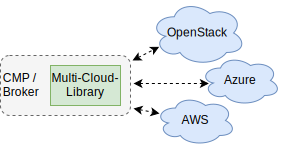
\includegraphics[width=0.48\textwidth]{images/multi-cloud-library.pdf}
	\def\svgwidth{0.75\textwidth}
	{\footnotesize \textsf{
			\includesvg{images/hyrise-r-deployment}}}
	\caption{Test-Deployment mit zwei Hyrise-R-Clustern, verteilt auf eine Public- und eine Private-Cloud. Orchestriert werden beide Services durch die selbstentwickelte Cloud-Management-Plattform aus der Private-Cloud heraus -- sie überwindet Provider- und Infrastrukturgrenzen.}	
	\label{fig:hyrise-r-deployment}
	%\end{wrapfigure}
\end{figure}

Der Dispatcher empfängt alle Anfragen an den Hyrise-R-Cluster. Jede Anfrage mit Schreibanteil leitet der Dispatcher an den Master-Knoten. Hier wird die Anfrage bearbeitet, in das Log geschrieben und anschließend mit allen Replicas synchronisiert. Enthält eine Anfrage nur Leseanteile, verteilt der Dispatcher sie an einen beliebigen Knoten.

% query performacne und synchronisations overhead.
Wir starten Hyrise-R immer als Cluster aus Dispatcher, Master und drei Replicas oder skalieren dynamisch je nach Leistungsanforderungen und SLO-Bedingungen.

1. Betrieb über Cloud-Grenzen hinweg
2. Betrieb auf heterogener Infrastruktur
3. Skalieren nach Leistungsanforderungen
4. Skalieren nach SLOs und Nutzeranforderungen
% Hier: Startzeit des Clusters als Metrik zur Bewertung des Brokerings. Stark abhängig von der Performance der Cloud-Infrastruktur und Netzwerverbindungen.
%Gemessen wird also nicht die Synchronisationszeit der Hyrise-R-Lösung, sondern die Skalierungsfähigkeiten der verwendeten Cloud-Lösungen und Orchestrierungstechniken.

HTTP-Schnittstelle empfängt Anfragen im JSON-Format: NoOp startet keine Datenbank-Operation, durchläuft aber alle Datenbankkomponenten von HTTP-Handling über Parser bis Executor.

Python-Code überarbeitet und parallelisiert.


Stattdessen wollen wir eine echte Anfrage Ausführen. Dazu nutzen wir die vorbereitete Beispieldatenbank und Anfrage aus einer früheren Arbeit.

Um sowohl OLTP- als auch OLAP-Fähigkeiten der In-Memory-Datenbank zu überprüfen, nutzen vorherige Arbeiten \cite{ssiclops:d42:experiments-measurements} den CH-benCHmark der TU München \cite{cole:2011:db-benchmark}. Dieser ist eine Mischung aus Transaktions- und Analysebenchmark, angelehnt an den hybriden Einsatz aktueller Datenbanksysteme in Unternehmen: Die gleichen Tabellen eines einzigen Datenbanksystems erfüllen alle Aufgaben des täglichen Geschäfts und liefern gleichzeitig umfassende Analysen. Trotzdem bleibt die Vergleichbarkeit des Benchmarks mit klassischen, getrennten Systemen.

Die Beispieldatenbank enthält eine Auftragshistorie mit knapp 300\,000 Datensätzen. Jede Zeile besteht aus sieben zufälligen Integer-, zwei String- und einem Float-Wert. So ergibt sich eine Rohgröße von 21,3\,MB. Die Beispielanfrage\footnote{\url{https://db.in.tum.de/research/projects/CHbenCHmark/}} liefert alle Bestellungen eines bestimmten Zeitraumes, sowie Summe, Gesamt- und Durchschnittswert aller enthaltenen Posten. Sie dient uns als \emph{Smoke-Test} -- liefert der Hyrise-R-Cluster eine valide Antwort im vorgegebenen Zeitrahmen, ist die generelle Funktionsfähigkeit gegeben und das Deployment erfolgreich abgeschlossen:

\begin{minted}{sql}
SELECT ol_number,
       SUM(ol_quantity) AS sum_qty,
       SUM(ol_amount)   AS sum_amount,
       AVG(ol_quantity) AS avg_qty,
       AVG(ol_amount)   AS avg_amount,
       COUNT(*)         AS count_order
FROM orderline 
WHERE ol_delivery_d > '2007-01-02 00:00:00.000000' 
GROUP BY ol_number
ORDER BY ol_number
\end{minted}


%Kosten: Rechenzeit und Bandbreite (außerhalb einer Cloud) also gegenläufiges Ziel zu Portabilität und Ausfallsicherheit, denn die geringsten Kosten fallen bei dem Betrieb in einer einzelnen Cloud eines Providers an.
%i) providers’ pricing models, (ii) application’s communication patterns and (iii) distribution of nodes over providers.
%https://www.google.de/url?sa=t&rct=j&q=&esrc=s&source=web&cd=1&ved=0ahUKEwju27vHs6DZAhUCWRQKHRv7BEcQFggrMAA&url=http%3A%2F%2Fwww.mikesmit.com%2Fwp-content%2Fpapercite-data%2Fpdf%2Fcloud2012.pdf&usg=AOvVaw3e6yhHYmhWBbIxtr7MqkuX

%verschiedene OpenStack-Versionen haben unterschiedliche Schnittstellen. Auch dies kann über die Middleware abgefangen werden. RefStack testet API, Rally testet performance und führt tempest-Tests aus.


Aufwand einer Multi-Cloud-Strategie

Umsetzung der Policys

Potential

Vorteile durch Multi-Cloud-Bibliotheken

Aufwand für ein Multi-Cloud-Testbed

Redundanz fehlt: Auch die CMP muss in einer vertrauenswürdigen Umgebung repliziert werden und synchronisieren. Dem Hyrise-R-Dispatcher fehlt diese Funktion ebenso.